\documentclass{extarticle}
\usepackage[14pt]{extsizes}
\usepackage{graphicx} % Required for inserting images
\usepackage[utf8]{inputenc}
\usepackage[T2A]{fontenc}
\usepackage[english,main=russian]{babel}
%\usepackage{lmodern}
%\usepackage{natbib}
\usepackage[center]{titlesec}
\usepackage{indentfirst}
\usepackage[left = 3cm, right = 1cm, top = 2cm, bottom = 2cm]{geometry}
\usepackage{tocloft} %пакет для оформления оглавления
\usepackage[nottoc]{tocbibind} %добавление списка источников в оглавление
\usepackage[titletoc]{appendix} %добавление приложений в оглавление
\usepackage{caption} %заголовки плавающих объектов
\usepackage{csquotes}
\usepackage{amsmath}
\usepackage{tikz}
\usepackage{braket}

\DeclareCaptionLabelSeparator{custom}{ -- }
\captionsetup[figure]{name=Рисунок, labelsep = custom}
\titleformat{\section}[hang]
{\normalfont\large\bfseries\filcenter}
{Глава \thesection.}{0.5em}{}
\pagestyle{myheadings}
%\bibliographystyle{gost-alphabetic.bbx}
%\usepackage[backend=biber, language=auto, style=gost-numeric]{biblatex}
%\titleformat{\section}[hang]{\normalfont\bfseries}{Глава \ \thesection .}{}
\usepackage[parentracker=true,backend=biber, hyperref=false, bibencoding=utf8, style=numeric, language=auto, autolang=other, sorting=none]{biblatex}
\addbibresource{library.bib}
\title{DIPLOMA 2}
\author{Евгений Музяев}
\date{May 2024}

\renewcommand{\baselinestretch}{1.25}
\renewcommand{\contentsname}{\normalsize {Список использованных источников}} 
%\renewcaptionname{\appendixname}{Приложение} 
%\renewcommand{\cftchapleader}{\cftdotfill{\cftdotsep}} 

\begin{document}
\begin{titlepage}
%\large 
\begin{spacing}{1}
    \begin{center}
	Министерство науки и высшего образования Российской Федерации\\Санкт-Петербургский Политехнический Университет Петра Великого \\ Физико-механический институт \\ \textbf{Высшая школа фундаментальных физических исследований} 
\end{center}
\begin{flushright}
\begin{tabular}{l}
Работа допущена к защите\\Директор ВШФФИ \vspace{0.3cm} \\
\underline{\hspace{3.5cm}} В. В. Дубов \vspace{0.5cm}\\
«\underline{\hspace{1cm}}»\underline{\hspace{3cm}} 2024 г.
\end{tabular}
\end{flushright}
\vspace{0.3cm}
{ \begin{center}
\vspace{0.3cm}
\MakeUppercase{\textbf{выпускная квалификационная работа \\ магистерская диссертация}}\\
\vspace{0.3cm}

\MakeUppercase{\textbf{Асимметрия Сиверса в полуинклюзивном глубоко неупругом рассеянии лептонов на поперечно поляризованном протоне}}
\\
\vspace{0.5cm}
по направлению подготовки 03.04.02 «Физика»
\\

Профиль $03.04.02\_03$ «Физика ядра и элементарных частиц в фундаментальных и медицинских исследованиях»
\end{center}
}
\vspace{0.3cm}

\begin{flushleft}
	Выполнил \\
	студент гр. 5040302/20301 \hspace{0.3cm} %\hspace{1.9 cm} 
	\hfill  Е.В. Музяев
	\vspace{0.5cm}
	
	
	Научный руководитель\\
	профессор ВШФФИ, д.ф.-м.н.
	\hspace{0.1 cm} \hspace{1.8 cm} 
	\hfill  {Я.А. Бердников}
	\vspace{0.5cm}
	
	Консультант \\
	по нормконтролю \hspace{2.1 cm} \hspace{2 cm} \hfill  {Д.О. Котов}
\end{flushleft}


\begin{center}
	Санкт-Петербург
\end{center}
\begin{center}
    2024
\end{center}
\end{spacing}

\end{titlepage}	



\newpage
\tableofcontents
\setcounter{page}{4}
\thispagestyle{headings}
\newpage


\section*{Введение}\addcontentsline{toc}{section}{Введение}
%\selectlanguage{russian}

До сих пор одним из важных вопросов современной физики является исследование спина нуклона. Как известно, нуклон состоит из кварков и связывающих их глюонов. В частности, особый интерес представляет то, как спин нуклона распределяется по кваркам и глюонам. Решение этой задачи позволяет понять устройство материи, а также исследовать эффекты, предсказываемые в рамках Стандартной Модели или найти новые эффекты вне неё. В решении этой проблемы огромную роль играет проведение экспериментов рассеяния лептонов (электронов, позитронов, мюонов) на адроне (например, протон или нейтрон) или на адронной системе (например, дейтрон). Несмотря на то, что первые подобные эксперименты были проведены в 50-х годах XX века Робертом Хофштедтером \cite{Hofstadter}, процесс глубоко неупругого рассеяния лептонов на нуклонных и ядерных мишенях до конца не изучен и представляет большой научный интерес.


Исследование характеристик глубоко неупругого рассеяния лептонов на нуклонной мишени позволяет рассматривать процессы, происходящие между частицами, из которых состоит нуклон. Возможно это благодаря размерам частицы-снаряда: лептоны обладают массой и размерами значительно меньшими, чем нуклоны. Например, размер электрона не превышает 0,0001 фемтометра (фм), в то время как размер протона составляет величину 0,74 фм \cite{Hofstadter}.


В 1968 году при проведении экспериментов по глубоко упругому рассеянию (ГНР) на линейном ускорителе электронов SLAC научной группой было установлено \cite{SLAC}, что неупругое сечение рассеяния практически не изменяется при изменении переданного импульса $Q^2$, что означает, что структурные функции практически не зависят от $Q^2$. Это явление получило название «скейлинг Бьёркена».


В 1969 году вышла статья Ричарда Фейнмана про партонную структуру частиц. Согласно партонной модели, при больших энергиях нуклоны состоят из безмассовых точечноподобных частиц – партонов. Таким образом, взаимодействие нуклонной материи при высоких энергиях можно представить в виде взаимодействия множества партонов, несущих долю импульса нуклона \cite{Feynman}. При этом предполагается, что импульс партонов коллинеарен импульсу нуклона. Распределение кварков по импульсу внутри нуклона можно описать партонной функцией распределения (ПФР).


В 1986 г. в эксперименте по рассеянию поляризованных µ-мезонов на поляризованных протонах в Европейской-мюонной коллаборации (EMC) был получен удивительный результат: суммарный спин валентных кварков даёт вклад, равный лишь 33\% от спина нуклона [4]. Данная проблема получила название «спиновый кризис». Для исследования этой проблемы были проведены эксперименты HERMES (HERA Spin MESurement) [5] и COMPASS (COmmon Muon Proton Apparatus for Structure and Spectroscopy) [6], в которых рассматривались явления полуинклюзивного (с рождением и регистрацией выделенного мезона) глубоко неупругого рассеяния (ПГНР) лептонов на поперечно поляризованном протоне. В результате этих экспериментов была обнаружена азимутальная асимметрия образовавшихся мезонов.


Азимутальная асимметрия – отношение разности сечений рассеяния образовавшихся адронов влево и вправо на одинаковые углы в одной плоскости к сумме тех же сечений [7]:
\begin{equation}
    A_N =\frac{d\sigma^\uparrow -d\sigma^\downarrow }{d\sigma^\uparrow +d\sigma^\downarrow },
\end{equation} 
где $A_N$ -- азимутальная асимметрия, $d\sigma^\uparrow$  – сечение образовавшихся адронов в левой плоскости, $d\sigma^\downarrow$  – в правой плоскости.


 В эксперименте по рассеянию пучка поляризованных протонов на поляризованной водородной мишени, проведённых коллаборацией E704 в лаборатории Ферми, было обнаружено, что азимутальная асимметрия образовавшихся $\pi^0$-мезонов растёт с увеличением поперечного импульса и переменной Фейнмана $x_F$, что не нашло объяснений в рамках коллинеарной пертурбативной квантовой хромодинамики (КХД) [8]. Для объяснения этого эффекта были предложены партонные функции распределения, и функции фрагментации (ФФ), зависящие от величины поперечного импульса кварков.

 
 Измерение неколлинеарных партонных функций распределения кварков и глюонов важно для исследования внутренней структуры нуклона. Существует несколько способов измерения: исследование процессов Дрелл-Яна, образования прямых фотонов и полуинклюзивного глубоко неупругого рассеяния. 

\textit{Целью работы} является моделирование расчёта односпиновой азимутальной асимметрии Сиверса образовавшихся адронов в глубоко неупругом рассеянии лептонов на нуклоне - мишени с использованием Монте-Карло генератора событий PYTHIA8 и плагина Stringspinner, учитывающего эффекты поляризации частиц. 

В Главе 1 представлено введение в кинематику глубоко неупругого рассеяния, в главе 2 рассмотрены основы партонной модели и поляризация кварков, в 3-ей главе рассмотрена фрагментация кварков,  в 4-ей главе -- азимутальные асимметрии в процессах глубоко неупругого рассеяния на поперечно поляризованной мишени, в 5-ой главе представлено моделирование процессов ГНР на поляризованной мишени в Монте-Карло генераторе PYTHIA8, в 6-ой главе произведён расчёт асимметрий Сиверса в процессах рассеяния неполяризованных лептонов на поперечно поляризованной мишени и представлены результаты этого расчёта.

\newpage
\section{Глубоко неупругое рассеяние}
Глубоко неупругое рассеяние – процесс неупругого взаимодействия лептона (электрона, мюона, нейтрино) с адроном (например, протон или нейтрон) или с адронной системой (дейтрон, литий), протекающего при энергетическом масштабе сильно большем, чем сумма масс покоя участников взаимодействия. Неупругость предполагает, что в результате взаимодействия могут образовываться частицы, т.е. число участников рассеяния не сохраняется. Схему реакции можно представить в виде
\begin{equation}
	l + N \rightarrow l' + X,
\end{equation}
где $l, l'$ -- лептон до и после взаимодействия, $N$ - адронная система-мишень, $X$ -- продукты реакции. Если регистрируется только один вид частиц (например, лептон), то канал такой реакции называется инклюзивным. В случае, когда ещё и регистрируется другой вид частиц (например, адрон), то такой канал реакции называется полуинклюзивным:
\begin{equation}
	l + N \rightarrow l' + h + X,
\end{equation}
где $h$ -- регистрируемая частица-адрон (к примеру, $\pi$-мезон). 
\subsection{Кинематика глубоко неупругого рассеяния}
Рассмотрим глубоко-неупругое рассеяние электрона на протоне в приближении однофотонного обмена (дальнейшие рассуждения по этой теме справедливы и для других частиц – мюонов и нейтронов). При таком приближении предполагается, что лептон с нуклоном обмениваются виртуальным фотоном. Обозначим импульс протона через $P$, начальный и конечный импульс электрона – через $k$ и $k'$. Тогда можно вычислить вектор импульса, переданный виртуальным фотоном адронной системе как $q=k-k'$. Вектор \textit{q} неинвариантен (его величина зависит от выбора системы координат), поэтому принято пользоваться инвариантным квадратом импульса $q^2=-Q^2$.

Если величина переданного импульса $Q^2$ велика, то кварк «излучается» из нуклона так, что мягкие процессы не смогут сбалансировать реакцию. В таком случае лептон передаст импульс не всему нуклону как целому, а определённому кварку. Но несмотря на это, мягкие процессы не исчезнут – будут образовываться глюоны и кварк-антикварковые пары, и цветной кварк преобразуется в бесцветные адронные струи. Такой процесс называется фрагментацией, о котором речь пойдёт позже.

Упрощённая диаграмма процесса глубоко неупругого рассеяния на кварковом уровне представлена на Рисунке \ref{fig:DIS}.


\begin{figure}[h]
    \centering
    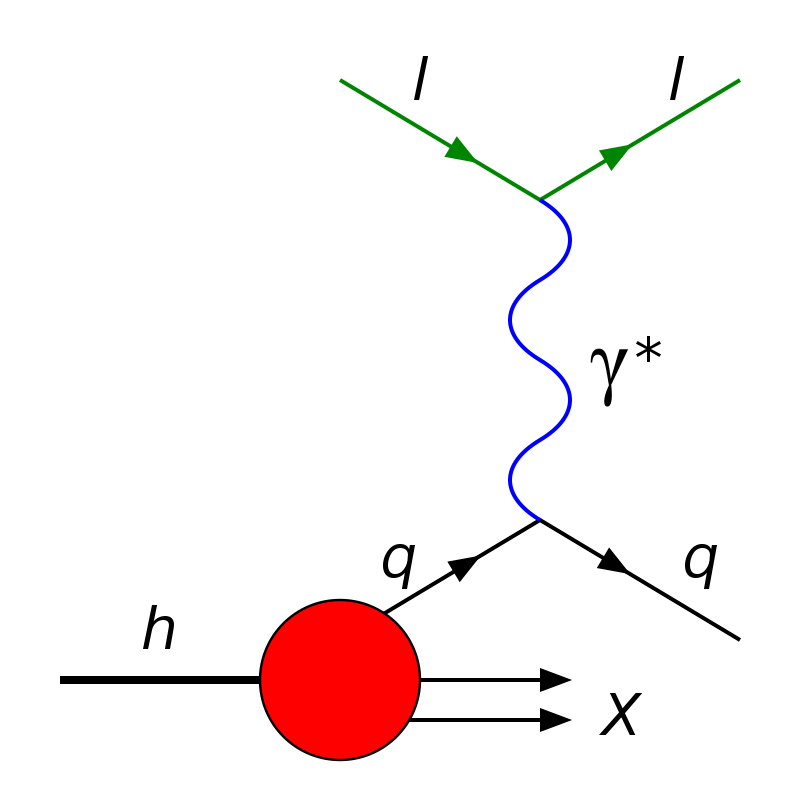
\includegraphics[width = 0.7\linewidth]{DIS.png}
    \caption{Упрощённая диаграмма глубоко неупругого рассеяния в приближении однофотонного обмена}
    \label{fig:DIS}
\end{figure}

Здесь налетающий лептон $l$ взаимодействует с кварком $q$ нуклона $h$, обмениваясь виртуальным фотоном $\gamma*$. Символом $X$ обозначены "остатки"\  адрона -- частицы, не участвующие в реакции.

Рассмотрим глубоко неупругое рассеяние электрона на протоне в системе центра масс. В этой системе электрон и протон будут лететь навстречу друг другу. Энергия в системе центра масс велика, поэтому массу протона можно игнорировать, следовательно, импульс протона будет подобен импульсу безмассовой частицы (фотона). Импульс составляющих протон кварков будет коллинеарен импульсу протона (практика показывает, что кварки обладают ненулевым поперечным импульсом). Таким образом, кварки будут нести часть импульса нуклона. Для описания этого вводится безразмерная переменная Бьёркена $x_{Bj}$, которая определяется как доля импульса нуклона, которую несёт кварк:
\begin{equation}
    x_{Bj}= \frac{Q^2}{2Pq},
\end{equation}
где \textit{P} -- импульс нуклона, \textit{q} -- переданный импульс. 
Таким образом, импульс \textit{p} кварка адрона \textit{h}, обладающего импульсом $P$, можно выразить как
\begin{equation}
    p=x_{Bj}P.
\end{equation}
По определению величина переменной Бьёркена положительна и не превышает единицы: 
\begin{equation}
    0 < x_{Bj} \leq 1.
\end{equation}
Переменная Бьёркена равняется единице в случае упругого рассеяния, если меньше единицы -- то неупругое. Существует случай, когда переменная Бьёркена больше единицы. Такое возможно в результате кумулятивного эффекта в ядро-ядерных рассеяниях.

Введём кинематическую переменную $y$, выражающую относительную потерю энергии налетающей частицы-лептона:
\begin{equation}
    y = \frac{P \cdot q}{P \cdot k},
\end{equation}
где $q$ -- импульс виртуального фотона, $k$ -- начальный импульс лептона, $P$ -- импульс адрона. По определению, переменная $y$ не может превышать единицы.

Потерю энергии налетающей частицы в системе центра масс можно выразить как 
\begin{equation}
    \nu = \frac{P \cdot q}{M},
\end{equation}
где $M^2 = P^2$ -- масса нуклона-мишени. Переменную Бьёркена можно выразить через эту величину:
\begin{equation}
    x_{Bj} = \frac{Q^2}{2M\nu}.
\end{equation}
Квадрат эффективной массы системы (cумма квадратов 4-импульсов системы):
\begin{equation}
	W^2 = (P+q)^2 = M^2 + 2M\nu - Q^2.
\end{equation}
Квадрат полной энергии лептона и нуклона (переменная Мандельштама $s$):
\begin{equation}
	s^2 = (k+P)^2 = M^2 + \frac{Q^2}{x_{Bj}y} + m_l^2 \approx M^2 + \frac{Q^2}{x_{Bj}y}, 
\end{equation}
т. к. $(M^2 \gg m_l^2)$, где $m_l$ -- масса лептона. 

В случае, когда регистрируются образующиеся в результате рассеяния адроны (инклюзивный канал), то в рассмотрение вводится переменная $z$, выражающая долю энергии нуклона, которую унёс адрон в конечном состоянии:
\begin{equation}
	\label{eq:z}
	z = \frac{P \cdot P_h}{P \cdot q} = \frac{E_h}{\nu},
\end{equation}
где $P_h$ -- импульс детектируемого адрона, $E_h$ -- энергия детектируемого адрона. 

Определённые выше кинематические переменные нужны для того, чтобы описать движение частиц до и после рассеяния, что помогает в анализе процессов, происходящих в результате ГНР. В анализе играет существенную роль сечение рассеяния, речь о котором пойдёт в следующем параграфе.
\subsection{Сечение глубоко неупругого рассеяния}
\subsubsection{Сечение рассеяния в приближении Мотта}
Физика элементарных частиц рассматривает процессы, происходящие на квантовомеханических масштабах. Изучение таких процессов требует вероятностного подхода описания событий. Одним из таких способов изучения взаимодействия элементарных частиц является нахождение дифференциального и интегрального сечений рассеяния. По величине сечения рассеяния можно определить вероятность того или иного процесса: распада, образования новых частиц и т.д. Чем больше величина сечения рассеяния, тем выше вероятность этого процесса.

Дифференциальное сечение рассеяния в лабораторной системе определяется следующим образом:
\begin{equation}
    \frac{d\sigma}{d\Omega}(\theta) = \frac{\frac{dN}{d\Omega}(\theta)}{I \cdot n},
\end{equation}
где $\theta$ -- угол рассеяния, $I$ -- поток налетающих частиц, $n$ -- число частиц мишени, $\Omega$ -- телесный угол, $\frac{dN}{d\Omega}$ -- число частиц, вылетевших в единичном элементе телесного угла $\Omega$ за единицу времени.

Полное (эффективное) сечение рассеяния можно получить, проинтегрировав по углу:
\begin{equation}
    \sigma = \int \frac{d\sigma}{d\Omega}d\Omega. 
\end{equation}
Эффективное сечение рассеяния характеризует вероятность взаимодействия налетающей частицы с частицей-мишенью. Полное эффективное сечение рассеяния складывается из сечений упругого (с сохранением числа частиц) рассеяния и неупругого (с образованием новых частиц):
\begin{equation}
    \sigma = \sigma_{el} + \sigma_{inel},
\end{equation}
где $\sigma_{el}$ -- сечение упругого рассеяния, $\sigma_{inel}$ -- сечение неупругого рассеяния. 

Рассмотрим дифференциальное сечение электрона на ядре с числом протонов $Z$, которое выражается как 
\begin{equation}
    \frac{d\sigma}{d\Omega} = ( \frac{d\sigma}{d\Omega})_{Mott} |F(q)|^2 ,
\end{equation}
где $\Omega$ -- телесный угол, $F(q)$ -- форм-фактор, $q = k-k'$ -- переданный импульс. Выражение в скобках означает сечение Мотта -- рассеяние электрона на точечной частице:
\begin{equation}
    (\frac{d\sigma}{d\Omega})_{Mott} = \frac{(Z\alpha)^2 E^2}{4k^4 \sin^4 (\theta/2)} (1- \frac{k^2}{E^2} \sin^2(\theta/2)),
\end{equation}
где $Z$ -- электрический заряд частицы, $\theta$ -- угол рассеяния, $E$ -- энергия рассеянной частицы. Таким образом, форм-фактор $F(q)$ возникает, когда частица-мишень является составной. Форм-фактор зависит от распределения составляющих ядро частиц и равен Фурье-образу плотности распределения электрического заряда:
\begin{equation}
    F(q) = \int \rho(r) \exp^{\frac{i}{\hbar}qr}dr,
\end{equation}
где $\rho(r)$ -- плотность распределения, $r$ -- радиус-вектор из центра ядра, $\hbar$ -- приведённая постоянная Планка.

В работе \cite{Breidenbach} было показано, что при увеличении энергии центра масс реакции происходит уменьшение упругой части рассеяния. На графике \ref{fig:Mott} показано отношение сечения рассеяния электрона на протоне к сечению Мотта при энергиях центра масс 2, 3, 3,5 ГэВ. Отдельной линией выделено сечение упругого рассеяния, которое падает с увеличением квадрата переданного импульса. Это говорит о том, что протон составная частица. 
\begin{figure}[h]
    \centering
    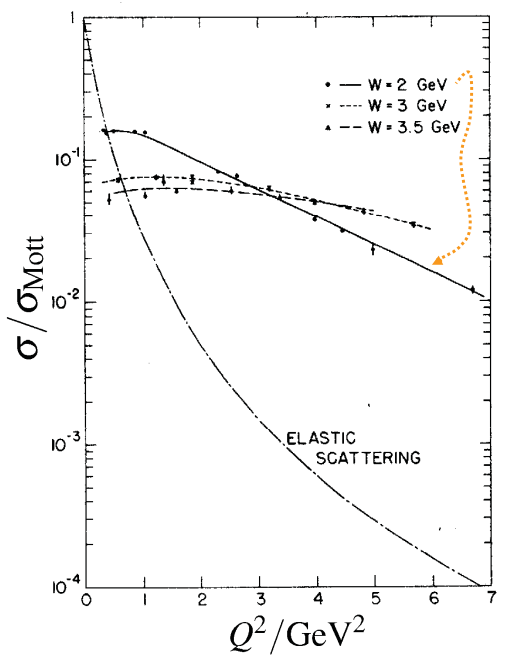
\includegraphics[width = 0.6\linewidth]{Mott.png}
    \caption{Отношение дифференциального сечения рассеяния по углу и энергии к сечению Мотта \cite{Breidenbach}}
    \label{fig:Mott}
\end{figure}

Однако поведение неупругого рассеяния показывает другие результаты -- его величина слабо зависит от $q^2$. Таким образом, сечение неупругого рассеяния приблизительно обладает единичным форм-фактором, что говорит о том, что электрон рассеивается на точечной частице, которая является составляющей нуклона.

\subsubsection{Расчёт сечения глубоко неупругого рассеяния}

Приведём расчёт сечения глубоко неупругого рассеяния в приближении однофотонного обмена. Согласно правилам Фейнмана, матричный элемент $\mathcal{M}$ диаграммы (Рисунок \ref{fig:DIS}) будет равен
\begin{equation}
	i\mathcal{M} = (ie)^2 \bar{u}(k')\gamma^\nu u(k) i \frac{-g_{\mu\nu}}{q^2} \braket{X | J_h^\nu | P},
\end{equation}
где $e$ -- заряд электрона, $u$ -- четырёхмерный вектор импульса лептона, $k$ -- импульс лептона до взаимодействия, $k'$ -- импульс лептона после взаимодействия, $\gamma^\nu$ -- гамма матрица Дирака, $i \frac{-g_{\mu\nu}}{q^2}$ -- фотонный пропагатор, $ J_h^\nu $ -- адронный ток, $X$ -- адрон, $P$ -- импульс адрона. Величина в пропагаторе $g_{\mu\nu}$ есть метрический тензор пространства Минковского, представимый в виде диагональной матрицы:
\begin{equation}
	g^{\mu\nu} = g_{\mu\nu} = \begin{bmatrix} 1&0&0&0\\0&-1&0&0\\0&0&-1&0\\0&0&0&-1 \end{bmatrix}.
\end{equation}

Дифференциальное сечение рассеяния, усреднённое по спинам частиц, будет равно

\begin{equation}
	d\sigma = \frac{1}{4E' m_H} \frac{d^3k'}{(2\pi)^3 \cdot 2E'} \sum_X (2\pi)^4 \delta^4(q+P-xP) \cdot \frac{1}{2} \sum_{spin} |\mathcal{M}|^2,
\end{equation}
где $m_H$ -- масса адрона, $E$ -- энергия лептона до взаимодействия, $E'$ -- энергия лептона после взаимодействия,  $\delta^4$ -- четырёхмерная дельта-функция импульсов. Квадрат матричной амплитуды, усреднённый по спинам, будет равен
\begin{equation}
	\sum_{spin} |\mathcal{M}|^2 = \frac{e^4}{(q^2)^2}L_{\nu \mu}\braket{P | J_h^\nu | X} \braket{X | J_h^\mu | P}, 
	\label{eq:lepton}
\end{equation}
где $L_{\nu\mu}$ -- лептонный тензор:
\begin{equation}
	L_{\nu\mu} = 4 (k_\nu k'_\mu + k_\mu k'_\nu - g_{\nu\mu}k\cdot k').
\end{equation}
Введём тензор $W^{\mu\nu}$, который будет равен
\begin{equation}
	W^{\mu\nu} = \frac{1}{4\pi} \sum_X (2\pi)^4 \delta^4(q+P-xP) \braket{P | J_h^\nu | X} \braket{X | J_h^\mu | P}.
\end{equation}
Выражение выше называется адронным тензором. Тогда сечение рассеяния, проинтегрированное по импульсу рассеянного лептона $k'$, можно представить как свёртку лептонного и адронного тензоров:
\begin{equation}
	\frac{d\sigma}{d^3 k'} = \frac{e^4}{4\pi^2(Q^2)^2} \frac{1}{8EE'm_H}L_{\nu\mu}W^{\mu\nu}.
\end{equation}

Используя закон сохранения электрического заряда:
\begin{equation}
	(xP-P)_\mu \braket{X | J_h^\mu | P} = 0,
\end{equation}
получаем, что 
\begin{equation}
	q_\mu W^{\nu \mu} = q_\nu W^{\mu \nu} = 0. 
\end{equation}
С помощью этого уравнения можно определить ковариантную форму адронного тензора, которая будет равна
\begin{equation}
	W^{\nu \mu} = (-g^{\nu\mu}+ \frac{q^\nu q^\mu}{q^2})W_1 + (P^\nu - \frac{P\cdot q}{q^2}q^\nu)(P^\mu - \frac{P\cdot q}{q^2} q^\mu) W_2,
\end{equation}
где $W_1, W_2$ -- структурные функции адрона H, состоящего из точечноподобных партонов:
\begin{equation}
\begin{split}
	& W_1  =   \frac{Q^2}{4m^2} \delta(\nu - \frac{Q^2}{2m}), \\
	& W_2  =  \delta(\nu - \frac{Q^2}{2m}),
\end{split}
	\label{eq:deltastruct}
\end{equation}
где $\delta$ -- дельта-функция, $m$ -- масса партона. Функции $W_1, W_2$ зависят от квадрата энергии виртуального фотона $Q^2$ и потери энергии лептона $\nu$.

Дифференциальное сечение рассеяния глубоко неупругого рассеяния электрона на протоне в системе покоя протона будет равно
\begin{equation}
	\frac{d^2\sigma}{dE' d cos\theta} = \frac{8\pi \alpha^2}{Q^4} E'^2 (2W_1(q^2, \nu) \sin^2 (\theta /2) + W_2 (q^2, \nu) \cos^2 (\theta/2)),
\end{equation}
где $\theta$ -- угол рассеяния, $E'$ -- энергия рассеянного электрона.
\newpage
\section{Партонная модель}
Партонная модель описывает процессы, которые происходят внутри ядер и адронов. Основой партонной модели служит утверждение, что при энергиях сильно больших, чем инвариантная масса нуклона, взаимодействие между элементарными частицами можно представить через взаимодействие множества партонов. Таким образом, партон -- точечноподобная безмассовая частица, несущая долю импульса адрона. Как правило, партоны отождествляют с кварками и глюонами. 
Исходя из вышесказанного, нуклон при $Q^2 \gg M^2$ (предел Бьёркена) можно представить в виде "шубы"\ из множества кварков и глюонов, которые в том числе взаимодействуют между собой путём обмена глюонами.


Переменные на партонном уровне обычно обозначаются со специальным символом "\ $\hat{}$ " ("шляпка"). Введём переменные Мандельштама на партонном уровне в системе центра инерции:
\begin{equation}
\begin{split}
	& \hat{s} = (p_1+p_2)^2 = (k + xP)^2, \\
	& \hat{t} = (p_1-p_3)^2 = (k-k')^2 = -q^2, \\
	& \hat{u} = (p_2-p_3)^2 =(xP-k')^2= \hat{s} (1-y),
\end{split}
\end{equation}
где $p_1, p_2$ -- импульсы лептона и партона соответственно, $p_3, p_4$ -- импульсы лептона и партона после взаимодействия. Переменные Мандельштама являются инвариантами. 

Партонное дифференциальное сечение рассеяния электрона на кварке нуклона будет равно
\begin{equation}
	\frac{d\sigma}{d\hat{t}} = \frac{2\pi \alpha^2}{\hat{s}^2} \frac{\hat{s}^2 + \hat{u}^2}{\hat{t}^2},
\end{equation}
где $\alpha$ -- константа электромагнитного взаимодействия. 

\subsection{Скейлинг Бьёркена и структурные функции}

В 1968 году Дж. Бьёркен предположил, что в пределе $Q^2$ на бесконечности, структурные функции должны зависеть только от переменной Бьёркена $x_{Bj}$:
\begin{equation}
	\begin{split}
	MW_1(q^2, \nu) = F_1 (x) ,\\
	W_2(q^2, \nu) = F_2(x),
	\end{split}
	\label{eq:struct}
\end{equation}
где  $W_1, W_2$ -- структурные функции партонов в зависимости от переданного импульса, $F_1, F_2$ -- структурные функции, зависящие от переменной Бьёркена, $M$ -- масса нуклона, $x \equiv x_{Bj}$ -- переменная Бьёркена. Здесь и далее будем использовать именно это обозначение переменной Бьёркена для краткости формул.

Структурные функции зависят от величины спина. Рассмотрим случай полуцелого спина партонов и найдём соотношение между функциями $F_1$ и $F_2$. Для этого воспользуемся определением этих функций, используя соотношение (\ref{eq:struct}):
\begin{equation}
	\frac{F_1(x)}{F_2(x)} = \frac{MW_1(q^2, \nu)}{W_2(q^2, \nu)},
	\label{eq:frelation}
\end{equation}
с учётом того, что рассеяние происходит на точечной частице и тем самым, структурные функции представимы в виде дельта-функций (\ref{eq:deltastruct}), получаем
\begin{equation}
	\frac{W_1(q^2, \nu)}{W_2(q^2, \nu)} = \frac{Q^2}{4m^2},
\end{equation}
где $m = xM$ -- масса партона. Тогда соотношение (\ref{eq:frelation}) будет равно
\begin{equation}
	\frac{F_1(x)}{F_2(x)} =  \frac{Q^2}{4m^2} \frac{M}{\nu} =  \frac{Q^2}{2M\nu} \frac{1}{2x^2} = \frac{1}{2x},
\end{equation}
и в результате получаем соотношение Каллана-Гросса \cite{Callan-Gross}:
\begin{equation}
		F_2(x) = 2xF_1(x).
\end{equation}
Таким образом, безразмерные структурные функции $F_1, F_2$ зависимы. В случае, когда спин партонов нулевой, то структурные функции тоже равны нулю:
\begin{equation}
	F_1 (x) = 0.
\end{equation}

Численно выразить безразмерные структурные функции можно через партонные функции распределения.

\subsection{Партонные функции распределения}
Поведение кварков в нуклоне можно описать партонной функцией распределения $f(x,Q^2)$ – плотности вероятности обнаружить в адроне партон, обладающего долей импульса $x$ при энергетическом масштабе взаимодействия $Q^2$. Вследствие того, что ПФР есть плотность вероятности, то сумма ПФР по всем партонам даёт единицу (импульс нуклона):
\begin{equation}
	\sum_i \int_0^1 x f_i(x)dx = 1.
\end{equation}
Вычислить ПФР можно только исходя из экспериментальных данных с помощью операции фитирования (нахождения функции аппроксимации, максимально соответствующей экспериментальной кривой). 

Сечение рассеяния лептона на нуклоне можно представить в виде суммы партонных сечений по всем партонам, помноженных на функции распределения соответствующих партонов:
\begin{equation}
	\sigma = \int_0^1 dx_q f_q(x_q) \hat{\sigma},
\end{equation}
где $x_q$ -- доля импульса кварка $q$, $\hat{\sigma}$ -- партонное сечение рассеяния.
Партонные функции распределения разделяют на коллинеарные (импульс партона сонаправлен с импульсом адрона) и неколлинеарные (партоны имеют ненулевую составляющую поперечного импульса).
\subsubsection{Коллинеарные партонные функции}
Рассмотрим коллинеарные ПФР. Структурные функции равны сумме плотностей партонов, составляющих нуклон:
\begin{equation}
F_2(x) = \sum_i e^2_i x f_i(x),
\end{equation}
где $e_i$ -- электрический заряд $i$-го партона.



\newpage
\subsection{Поляризация частиц}

 В физике достаточно изучена электромагнитная поляризация волн – направленное в определённой плоскости колебание векторов \textbf{E} и \textbf{H}. Поляризация частиц имеет другую природу и выражается в преимущественной ориентации спина частицы вдоль выбранного направления по отношению к её импульсу. Поляризацию частиц разделяют на поперечную (спин частицы перпедикулярен её импульсу) и продольную (спин частицы коллинеарен импульсу). 
 Охарактеризовать поляризацию частицы можно через спиральность:
 \begin{equation}
     h = \frac{\textbf{S} \cdot \textbf{P}}{|S|\cdot |P|}
 \end{equation}
%h=(S⃗⋅P⃗)/(|S⃗|⋅|P⃗|) ,
где \textbf{S} – вектор спина частицы, \textbf{P} – вектор импульса. Если спиральность частицы по модулю равняется единице, то она поляризована продольно, если спиральность равна нулю, то поперечно. 

Поляризацию релятивистской частицы можно выразить в виде векторного оператора поляризации (оператора Паули-Любански):
\begin{equation}
	W^\mu = \epsilon^{\mu\nu\rho\lambda}S_{\rho\lambda}\hat{p}_\nu,
\end{equation}
где $\mu, \nu, \rho, \lambda = 0, 1, 2, 3$, $\hat{p}_\nu$ -- 4-импульс частицы, $S_{\rho\lambda}$ -- спиновая матрица:
\begin{equation}
	S_{\rho\lambda} = (S, iS) \equiv \begin{pmatrix}
		0&S_x&S_y&S_z\\-S_x&0&-iS_z&iS_y\\-S_y&iS_z&0&-iS_x\\-S_z&-iS_y&iS_x&0
	\end{pmatrix},
\end{equation}
где $S$ -- матрица спина.


 Величина спина нуклона общеизвестна – 1/2, но до сих пор неизвестно распределение спина нуклона по его составляющим (конституэнтам), или, что аналогично, из чего складывается этот спин. До публикации результатов коллаборации EMC [4] считалось, что спин нуклона полностью складывается из спинов валентных кварков (те кварки, которые определяют квантовые числа адронов). Данный эксперимент показал, что валентные кварки дают вклад, равный лишь трети от суммарного спина. На данный момент достоверно известно, что спин в том числе распределяется по валентным кваркам, морским кваркам, глюонам и орбитальным моментам этих частиц. На рисунке \ref{fig:nucleo} схематично представлена картина возможного распределения спина нуклона по его составляющим.
 Однако, как оказалось, недостающие 70\% спина зависят не только лишь от орбитального момента кварков и глюонов \cite{Hagler}, и существует ненулевая корреляция между направлением спина партонов и их импульсов в нуклоне. 

\begin{figure}[ht]
    \centering
    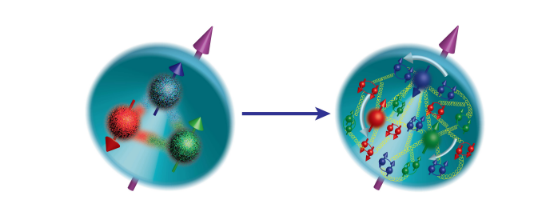
\includegraphics[width = 0.9\linewidth]{nucleo.png}
    \caption{Схематичное изображение эволюции представлений о внутренней структуре спина нуклона: слева – устаревшее представление, справа – современное представление}
    \label{fig:nucleo}
\end{figure}
 
 Вследствие этого, необходимо учитывать поперечный импульс партонов. Для этого в партонную функцию распределения вводится множитель, зависящий от величины поперечного импульса $k_{\perp}$:
 \begin{equation}
 	f(x, k_{\perp})dx =g(k_{\perp}) f(x) dx d^2k_{\perp},
 \end{equation}
 где множитель $g(k_{\perp})$ представим в виде гауссового пакета:
 \begin{equation}
 	g(k_{\perp}) = \frac{\exp [-k^2_{\perp} / \braket{k^2_\perp}]}{\pi \braket{k^2_\perp}}.
 \end{equation}

 В лидирующем порядке квантовой хромодинамики поляризованный нуклон можно описать тремя ПФР кварков – функцией $f_1^q$, которая показывает распределение неполяризованных кварков в неполяризованном нуклоне, спиральностью $g_1^q$, которая описывает кварки с продольной поляризацией в продольно поляризованном нуклоне, и «трансвёрсити» (поперечная поляризация) $h_1^q$, которая описывает распределение поперечно поляризованных кварков в поперечно поляризованном нуклоне \cite{Hagler}. Среди этих трех неколлинеарных партонных функций распределения «трансвёрсити» является менее изученной и наиболее труднодоступной из-за её киральной нечетной природы. Киральная нечётность означает, что при зеркальном отображении системы относительно оси координат симметрия системы не будет сохраняться.
Для измерения функции «трансвёрсити» необходимо изучение процесса, в котором участвуют две кирально-нечётные функции. Такую возможность даёт изучение азимутальных асимметрий адронов в полуинклюзивном глубоко неупругом рассеянии на поперечно поляризованной мишени. 


\begin{figure}[h]
	\centering
	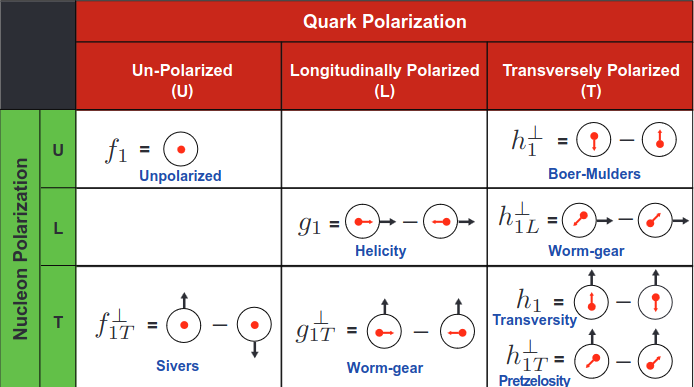
\includegraphics[width=\linewidth]{functions.png}
	\caption{Схематичное изображение партонных функций лидирующего твиста в проекции на плоскость реакции}
	\label{fig:functions}
\end{figure} 
Здесь большой круг обозначает нуклон, чёрная точка -- кварк, стрелки обозначают направления спина нуклона и кварка.

\subsection{Адронизация}
Результатом глубоко неупругого рассеяния является образование большого числа наблюдаемых частиц-адронов. Так как свободные партоны не наблюдаются в эксперименте, то должен существовать процесс, с помощью которого образовавшиеся в результате жёсткого взаимодействия партоны превращаются в адроны. Такой процесс называется адронизацией. Существует несколько моделей адронизации  \cite{Hadronization}:
\begin{itemize}
\item Фрагментация струн (используется генератором событий PYTHIA);
\item Фрагментация кластеров (используется генератором событий HERWIG);
\item Независимая фрагментация (устаревшая модель, предложенная Фейнманом).
\end{itemize}
 
Процесс возникновения бесцветных адронов (частиц-участников ядерного взаимодействия) из цветных кварков называется фрагментацией. Так, дифференциальное сечение образование адрона в рассеянии электрона на протоне в зависимости от переменной $z$ (см. (\ref{eq:z})) будет пропорционально следующей сумме:
\begin{equation}
	\frac{d\sigma(ep \rightarrow hX)}{dz} \propto \sum_q e_q^2 f_q (x) D_h^p(z),
\end{equation}
где $e_q$ -- электрический заряд кварка $q$, $f_q (x)$ -- партонная функция распределения кварка $q$ в протоне $p$, $D_h^p(z)$ -- функция фрагментации, описывающая вероятность того, что партон $q$, несущий долю импульса $z$, фрагментирует в адрон $h$. Значение функции фрагментации можно определить только из эксперимента.

Одной из самых развитых моделей адронизации является модель фрагментации струн (модель адронизации Лунда). Рассмотрим данную модель.
\subsubsection{Модель адронизации Лунда}
Лундовская модель адронизации предполагает, что наблюдаемые частицы-адроны образуются в результате фрагментации (разрыва) цветных кварк-антикварковых струн. Возникновение струн связано с явлением цветового конфайнмента - удержания цветовых кварков и глюонов в бесцветных адронах. Экспериментально не наблюдалось свободных частиц, обладающих цветом. Таким образом, кварки находятся в связанном состоянии, между которыми натягивается глюонная струна. 

Согласно модели квантовой хромодинамики (КХД), конфайнмент возникает в результате того, что линейный член потенциала КХД между двумя цветными кварками (цветовой синглет) доминирует при больших расстояниях:
\begin{equation}
	V_{QCD}\approx \frac{4}{3} \frac{\alpha_s}{r} + \kappa r,
\end{equation}
где $\alpha_s$ -- константа сильного взаимодействия, $r$ -- расстояние между кварками, $\kappa \approx 1$ ГэВ/фм. 


Фрагментацию струн удобно представить в виде йо-йо модели. 

\begin{figure}[ht]
    \centering
    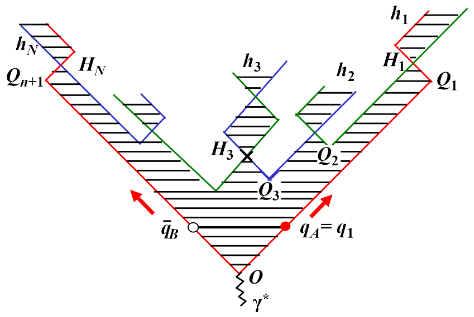
\includegraphics[width = 0.8\linewidth]{fragmentation.png}
    \caption{Схематичное изображение процесса адронизации \cite{LUND}}
    \label{fig:hadronization}
\end{figure} 

Здесь \textbf{O} – точка взаимодействия партона $q_A$ с виртуальным фотоном $\gamma*$, с которой начинается процесс адронизации; $\textbf{Q}_i$ – точки(узлы) разрыва струны, где $i = 1, 2, \dots, n$; \textbf{H} -- точки образования адронов $h_i$, где $i = 1, 2, \dots, n$.

Процесс начинается со взаимодействия виртуального фотона $\gamma*$, испущенного налетающим лептоном, с партоном мишени \textit{q} (здесь и далее предполагается, что взаимодействуют кварки, но последующие рассуждения справедливы и для глюонов). Виртуальный фотон передаёт кварку $A$ импульс, вследствие чего кварк $q_A$ начинает отдаляться от кварка $B$ оставшегося «раненого» нуклона. 

Между кварками A и B образуется струна, энергия которой растёт по мере отдаления кварков друг от друга. Струна может «порваться», когда её энергии становится достаточно для рождения кварк-антикварковой пары. Вероятность этого растёт со временем. Новообразовавшаяся пара ведёт себя аналогично паре-родителю, тем самым запускается многократный процесс, который продолжается до тех пор, пока это позволяет закон сохранения энергии-импульса. В результате многократного процесса струны теряют свою энергию, и кварки образуют связанные состояния – адроны. 

Для кварк-антикварковой пары справедлива следующая параметризация функции фрагментации
\begin{equation}
	f(z) \propto (1-z)^{a/z} exp(- \frac{b m_h}{z}),
\end{equation}
где $m_h$ – масса адрона, параметры $a$ и $b$ настраиваются в соответствии с экспериментальными данными. Таким образом, функция $f(z)$ показывает вероятность образования адрона массой $m_h$ с долей импульса $z$, полученной от остатка системы.
\subsubsection{Модель 3P0}
\newpage
\section{Азимутальные асимметрии}
\subsection{Полуинклюзивное глубоко неупругое рассеяние}
Одним из способов исследования внутренней структуры нуклона является изучение полуинклюзивного глубоко неупругого рассеяния. В зависимости от кинематических характеристик рождающихся частиц (например, распределения частиц по энергии) можно сказать о характере взаимодействия частиц, из которых состоит адрон. 

Особый интерес представляет изучение ПГНР неполяризованного лептона на поперечно поляризованной мишени. Удобно схематично обозначать ПГНР в виде трёхмерной диаграммы (Рисунок \ref{fig:sidis}):
\begin{figure}[h]
	\centering
	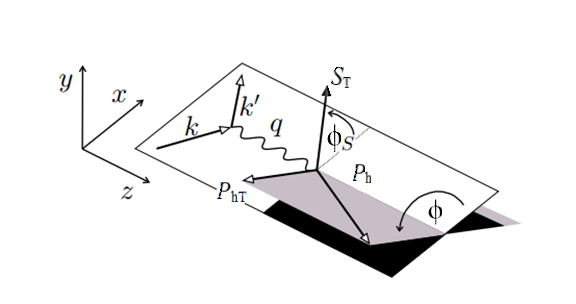
\includegraphics{sidis.png}
	\caption{Трёхмерная схема ПГНР неполяризованного лептона на поперечно поляризованном адроне в системе центра покоя мишени.}
	\label{fig:sidis}
\end{figure} \\
Здесь $k$ -- импульс лептона до обмена виртуальным фотоном, $k'$ -- импульс лептона после взаимодействия, $q = k-k'$ -- импульс виртуального фотона, $P_h$ -- импульс вылетающего адрона, $P_{hT}$ -- поперечный импульс вылетающего адрона, $S_T$ -- вектор спина поперечной поляризации, $\phi$ -- азимутальный угол между плоскостью реакции и плоскостью вылетающего адрона, $\phi_S$ -- азимутальный угол между вектором поляризации и плоскостью реакции. Азимутальный угол $\phi_h$ задаётся следующими соотношениями:
\begin{equation}
	\begin{split}
		\cos \phi_{h} = \frac{\hat{\textbf{q}} \times \textbf{k}}{|\hat{\textbf{q}} \times \textbf{k}|} \cdot \frac{\hat{\textbf{q}}\times \textbf{P}_h}{|\hat{\textbf{q}}\times \textbf{P}_h|}, \\
		\sin \phi_{h} = \frac{(\textbf{k}\times \textbf{P}_h)\cdot \hat{\textbf{q}}}{|\hat{\textbf{q}} \times \textbf{k}|\cdot|\hat{\textbf{q}}\times \textbf{P}_h|}, \\
	\end{split}
\end{equation}
где $\hat{\textbf{q}} = \frac{\textbf{q}}{|\textbf{q}|}$ -- трёхмерный вектор импульса кварка, величины $\textbf{P}_h, \textbf{k}$ заданы выше. 

Кроме объявленных выше кинематических переменных, часто вводят углы $\psi$ -- азимутальный угол спина мишени вокруг направления пучка лептонов и $\theta$ -- угол между импульсом лептона $k$ и кварка $q$ \cite{Diehl}. Угол $\theta$ можно выразить следующим образом:
\begin{equation}
	\sin \theta = \gamma \sqrt{\frac{1-y-\frac{1}{4}y^2 \gamma^2}{1+\gamma^2}},
\end{equation} 
где $\gamma$ -- кинематический фактор, который выражается как:
\begin{equation}
	\gamma = \frac{2Mx}{\sqrt{Q^2}}.
\end{equation}
Азимутальный угол $\psi$ будет равен
\begin{equation}
	\begin{split}
		 & \sin \psi = \frac{\cos \theta \sin \phi_S}{\sqrt{1-\sin^2 \theta \sin^2 \phi_S}}, \\
		 & \cos \psi = \frac{\cos \phi_S}{\sqrt{1-\sin^2 \theta \sin^2 \phi_S}}.
	\end{split}
\end{equation}
В кинематике ГНР величина $\gamma$ мала, поэтому
\begin{equation}
	\sin \theta \approx \gamma \sqrt{1-y},
\end{equation}
а азимутальный угол $\psi \approx \phi_S$.

Вектор поляризации $\textbf{S}$ можно параметризовать как
\begin{equation}
	\textbf{S} = \begin{pmatrix}
			S_T \cos \phi_S \\ S_T \sin \phi_S\\ -S_L \\ 
	\end{pmatrix}.
\end{equation}
В случае поперечной поляризации $S_L = 0$.


Рассмотрим дифференциальное сечение ПГНР неполяризованного мюона на поперечно поляризованном протоне. Определить сечение в первом разложении можно с помощью правил Фейнмана:
\begin{equation}
\begin{split}
	& d\sigma = \frac{1}{4k\cdot P_X} \sum_{s_k'} \sum_X \int \frac{d^3 P}{(2\pi)^3 2 E_X} \\
	& \times (2\pi)^4 \delta^4(P+k-P_X - P_h - k')|\mathcal{M}^2| \frac{d^3 k'}{(2\pi)^3 2E'}\frac{d^3 P_h}{(2\pi)^3 2E_h}, \\
\end{split}
\end{equation}
где суммирование проводилось по спинам рассеянных лептонов $s_k'$, $P_X$ -- импульс "оставшейся"\ части протона, $E_X$ -- энергия этой части. Квадрат амплитуды матричного элемента будет равен
\begin{equation}
		|\mathcal{M}^2| = \frac{e^4}{q^4} (\bar{u}_k'\gamma_\mu u_k)^{*}(\bar{u}_k'\gamma_\nu u_k)  \braket{X, P_h S_h | J_h^\mu (0) | PS}^{*} \braket{X, P_h S_h | J_h^\nu (0) | PS},
\end{equation}
где $S$ -- вектор поляризации адрона, * означает эрмитовое сопряжение. По аналогии с выражением \ref{eq:lepton} можно ввести лептонный тензор $L_{\mu \nu}$ \cite{Barone_2002}:
\begin{equation}
	L_{\mu \nu} = \sum_{s_{k'}} (\bar{u}_k'\gamma_\mu u_k)^{*}(\bar{u}_k'\gamma_\nu u_k),
\end{equation}
а адронный тензор $W^{\mu \nu}$ равен:
\begin{equation}
	\begin{split}
		W^{\mu \nu} = \frac{1}{(2\pi)^4} \sum_X \int \frac{d^3 P}{(2\pi)^3 2 E_X} (2\pi)^4 \delta^4(P+k-P_X - P_h - k') \\
		\times \braket{X, P_h S_h | J_h^\mu (0) | PS}^{*} \braket{X, P_h S_h | J_h^\nu (0) | PS}.
	\end{split}
\end{equation}
Таким образом, дифференциальное сечение можно представить в виде свёртки лептонного и адронного тензоров:
\begin{equation}
	d\sigma = \frac{1}{4k\cdot P_X} L_{\mu\nu}(s_k) W^{\mu \nu}(S_h) \frac{d^3 k'}{(2\pi)^3 2E'}\frac{d^3 P_h}{(2\pi)^3 2E_h}.
\end{equation}
Перейдём к инвариантным безразмерным переменным:
\begin{equation}
	\frac{d\sigma}{dxdydzd\phi dP^2_{hT}d\phi_S} = \frac{e^2 y}{8zQ^4}2MW^{\mu\nu}L_{\mu\nu},
\end{equation}
где $x,y,z$ заданы в уравнениях (\ref{eq:z}).

Следуя теореме о факторизации, полное сечение ПГНР можно выразить в виде суммы функций факторизации:
\begin{multline} 
	\label{sigma}
	\frac{d\sigma}{dx dy d \psi dz d \phi_{h} dP^{2}_{h \perp}} = \\
	= \frac{\alpha^2}{xy Q^{2}} \frac{y^2}{2 (1 - \varepsilon)} \left(1 + \frac{\gamma^2}{2x} \right)
	\Biggl \lbrace F_{U U, T} +
	\varepsilon F_{U U, L} +
	\sqrt{2 \varepsilon (1 + \varepsilon)} \cos \phi_h F_{UU}^{\cos \phi_h} + \\
	+ \varepsilon_e \cos(2\phi_h) F_{U U}^{\cos 2\phi_h} +
	\lambda_e \sqrt{2 \varepsilon (1 - \varepsilon)} \sin \phi_h F_{L U}^{\sin \phi_h} + \\
	+ S_{} \left [ \sqrt{2 \varepsilon (1 + \varepsilon)} \sin \phi_h F_{UL}^{\sin \phi_h} +
	\varepsilon \sin(2\phi_h) F_{UL}^{\sin 2\phi_h} \right] + \\
	+ S_{} \lambda \left [ \sqrt{1 - \varepsilon^2} F_{L L} +
	\sqrt{2 \varepsilon (1 - \varepsilon)} \cos \phi_h F_{LL}^{\cos \phi_h} \right] + \\
	+ |\vec S_{\perp}| \Biggl[ \sin(\phi_h - \phi_S) \left(F_{U T, T}^{\sin(\phi_h - \phi_S)} +
	\varepsilon F_{UT, L}^{\sin(\phi_h - \phi_S)} \right) + \\
	+ \varepsilon \sin(\phi_h + \phi_S) F_{U T}^{\sin (\phi_h + \phi_S)} +
	\varepsilon sin (3\phi_h - \phi_S) F_{UT}^{\sin (3\phi_h - \phi_S)} + \\
	+ \sqrt{2 \varepsilon (1 + \varepsilon)} \sin \phi_S F_{UT}^{\sin \phi_S} +
	\sqrt{2 \varepsilon (1 + \varepsilon)} \sin(2\phi_h - \phi_S) F_{UT}^{\sin(2\phi_h - \phi_S)}  \Biggr] + \\
	+ |\vec S_{\perp}| \varepsilon_e \Biggl[ \sqrt{1 - \varepsilon^2} \cos(\phi_h - \phi_S) F_{LT, T}^{\cos(\phi_h - \phi_S)} +
	\sqrt{2 \varepsilon (1 - \varepsilon)} \cos \phi_S F_{LT}^{\cos \phi_S} + \\
	+ \sqrt{2 \varepsilon (1 - \varepsilon)} \cos(2\phi_h - \phi_S) F_{LT}^{\cos(2\phi_h - \phi_S)}  \Biggr] \Biggr \rbrace,
\end{multline}
где $\epsilon$ -- отношение продольного и поперечного фотонных потоков:
\begin{equation}
	\epsilon = \frac{1-y-\frac{1}{4}y^2\gamma^2}{1-y+\frac{1}{2} y^2 +\frac{1}{4}y^2\gamma^2},
\end{equation}
нижний индекс структурных функций $U$ обозначает неполяризованный пучок, $L$ -- продольную поляризацию, $T$ -- поперечную поляризацию. Нижние индексы обозначают следующее: левый индекс -- поляризация пучка лептонов, правый - поляризация пучка мишени (например, индекс $UT$ обозначает неполяризованный пучок лептонов, который рассеивается на поперечно поляризованной мишени).

Сечение ПГНР неполяризованного пучка лептонов на поляризованной мишени будет равно:
\begin{multline}
	\frac{d\sigma}{dx dy d \psi dz d \phi_{h} dP^{2}_{h \perp}} = \\
	= \frac{\alpha^2}{xy Q^{2}} \frac{y^2}{2 (1 - \varepsilon)} \left(1 + \frac{\gamma^2}{2x} \right) \Biggl \lbrace 	
	 |\vec S_{\perp}| \Biggl[ \sin(\phi_h - \phi_S) \left(F_{U T, T}^{\sin(\phi_h - \phi_S)} +
	\varepsilon F_{UT, L}^{\sin(\phi_h - \phi_S)} \right) + \\
	+ \varepsilon \sin(\phi_h + \phi_S) F_{U T}^{\sin (\phi_h + \phi_S)} +
	\varepsilon sin (3\phi_h - \phi_S) F_{UT}^{\sin (3\phi_h - \phi_S)} + \\
	+ \sqrt{2 \varepsilon (1 + \varepsilon)} \sin \phi_S F_{UT}^{\sin \phi_S} +
	\sqrt{2 \varepsilon (1 + \varepsilon)} \sin(2\phi_h - \phi_S) F_{UT}^{\sin(2\phi_h - \phi_S)}  \Biggr]\Biggr \rbrace.
\end{multline}
\subsection{Асимметрия Коллинза}
\subsection{Асимметрия Сиверса}
Функцию распределения кварков в поперечно поляризованном протоне можно представить в виде разности ФР кварков в неполяризованном протоне и функции Сиверса:
\begin{equation}
	f_{q,p\uparrow} (x,k^2_T )=f_1^q (x,k^2_T )-f_{1T}^{\perp q} (x,k^2_T )(P\times k_T ) \cdot \frac{S_T}{M},
\end{equation}
где M – масса протона (938 МэВ/$c^2$), $k_T$ – поперечный импульс кварка, $f_{1q}$ – функция распределения кварков в неполяризованном протоне, $f_{1T}^{\perp q}$ – функция Сиверса, которая обозначает зависимость между поперечным импульсом «поражённого» кварка и поляризацией мишени. Индекс $\perp q$ означает то, что ПФР проинтегрирована по поперечному импульсу кварка, индекс 1 означает лидирующий твист.

Структурная функция Сиверса равняется свёртке функции Сиверса и неполяризованной функции фрагментации:
\begin{equation}
	F^{sin(\phi-\phi_S)}_{UT} = \mathcal{C}[-\frac{P\cdot p_T}{M}f_{1T}^{\perp q}D_1^{q \rightarrow h}]
\end{equation}


\newpage 
\section{Моделирование процессов в PYTHIA}
\subsection{Поляризация в PYTHIA}
\subsection{Расчёт асимметрии Сиверса}
\newpage
\section*{Заключение}
\addcontentsline{toc}{section}{Заключение}
\newpage
\printbibliography
\end{document}
